\documentclass[unicode,11pt,a4paper,oneside,numbers=endperiod,openany]{scrartcl}

\usepackage{amsmath}
\usepackage[table,xcdraw]{xcolor}
\usepackage{soul}
\sethlcolor{lightgray}
\usepackage{float}
\usepackage{tikz}
\usetikzlibrary{matrix}
\usepackage{amsfonts}

\input{assignment.sty}
\begin{document}


\setassignment
\setduedate{May 20, 2021, 12pm (midnight)}

\serieheader{High-Performance Computing Lab for CSE}
    {2021}
    {Student: Pascal Dominic Müller}
    {\\ \\ Discussed with: \\
        $\bullet$ Tarzis Maurer [tamaurer] \\
        $\bullet$ Zuzanna Herud [zherud] \\
    }
    {Solution for Project 6}
    {}
\newline

\assignmentpolicy

% -------------------------------------------------------------------------- %
% -------------------------------------------------------------------------- %
% --- Exercise 1 ----------------------------------------------------------- %
% -------------------------------------------------------------------------- %
% -------------------------------------------------------------------------- %

\section{Scientific Mathematical HPC Software Frameworks - The Poisson Equation [35 points]}

\paragraph{Note:} Instead of denoting a point in $\Omega$ with $(x, y)$ we
will switch to the notation $(x_1,x_2)=(x,y)$. This makes the derivation and
general notation clearer and avoids possible confusion with indices.
We further use $y=g$ for the seekd after function.

\subsection{Problem Statement: The Poisson Equation}



We solve the poisson equation on the 2 dimensional unit rectangle
$\Omega \subset \mathbb R^2=[0,1] \times [0,1]$ with vanishing dirichlet BC.
\begin{alignat}{3}
  -\Delta &g(x, y) &&= f(x, y) &&\text{  on  } \Omega = [0,1] \times [0,1]\\
          &g(x, y) &&= 0 &&\text{  on  } \partial \Omega
\end{alignat}

whereas $\Delta \equiv \frac{\partial^2}{\partial x^2} + \frac{\partial^2}{\partial y^2}$

\subsection{Discretization}

\subsubsection{Grid}
We discretize the domain $\Omega = [0,1]\times[0,1]$ into a set of $N+2 \times N+2$
points including the vanishing boundary.
I.e. we have a grid with points $(i,j), \quad i,j\in\{0,\dots, N+1\}$

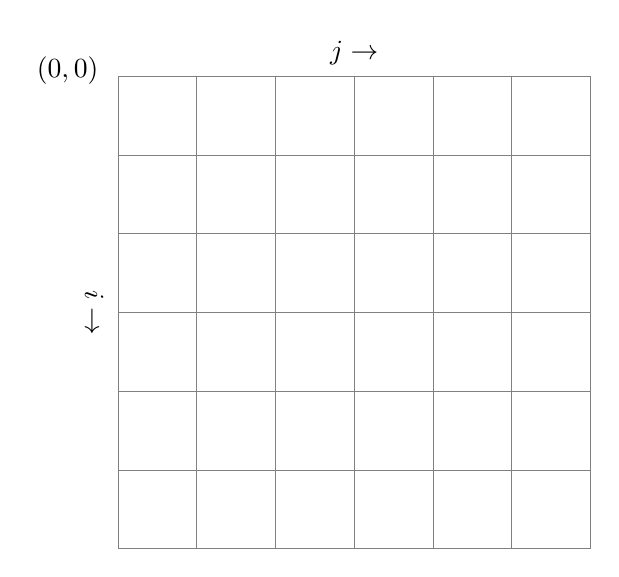
\begin{tikzpicture} 
  \draw[help lines] (0,0) grid (6,6);
  \node[anchor=center] at (3, 6.3) {$j \rightarrow$};
  \node[anchor=center, rotate=-90] at (-0.3, 3) {$i \rightarrow$};
  \node[label=below left:{$(0,0)$}] at (0,6.5) {};
\end{tikzpicture}


\subsubsection{Theory}
Let $g(x,y)$ be an at least twice continuous differentiable function. For the
discretization we use a central finite difference approach [1][Project 3].

The central finite difference in the direction of x (similar for y) is given by:

\begin{equation}
  \delta_h [g](x) = g(x+\frac{1}{2}h) - g(x-\frac{1}{2}h)
\end{equation}

which leads to

\begin{equation}
  \frac{\partial g(x)^2}{\partial^2 x} = \dots = 
    \frac{g(x + h) - 2g(x) + g(x - h)}{h^2}
\end{equation}

\subsubsection{LHS}
We first write out the laplacian operator.
\begin{equation}
  -\Delta g(x, y) = \frac{\partial g(x, y)^2}{\partial x^2} 
                      + \frac{\partial g(x, y)^2}{\partial y^2}
\end{equation}

Applying (4) to (5) for $x$ and $y$ separately, we get:
\begin{equation}
  \frac{\partial g(x, y)^2}{\partial x^2} = 
    \frac{g(x + h, y) - 2g(x, y) + g(x - h, y)}{h^2}
\end{equation}
\begin{equation}
  \frac{\partial g(x, y)^2}{\partial x^2} = 
    \frac{g(x, y + h) - 2g(x, y) + g(x, y - h)}{h^2}
\end{equation}

We plug (6) and (7) into (5) and use the notations (similar for $y$ and $j$)
\begin{itemize}
  \item $g(x, y) = g_{i,j}$
  \item $g(x + h, y) = g_{i+1, j}$
  \item $g(x - h, y) = g_{i-h, j}$
\end{itemize}

to end up with

\begin{align}
  -\Delta g^h(x,y) & = \frac{g(x + h, y) - 2g(x, y) + g(x - h, y)}{h^2} \\
                 &\ \ + \frac{g(x, y + h) - 2g(x, y) + g(x, y - h)}{h^2} \\
                 &= \frac{1}{h^2} ( g_{i+1,j} - 2g_{i,j} + g_{i-1,j}
                      + g_{i, j+1} - 2g_{i,j} + g_{i,j-1}) \\
                 &= \frac{1}{h^2} ( -4_{i,j} + g_{i+1,j} + g_{i-1,j}
                      + _{i, j+1} + g_{i,j-1} )
\end{align}

We get:

\begin{equation}
  \boxed{
      -\Delta g^h(x,y) = \frac{1}{h^2} ( -4g_{i,j} + g_{i+1,j} + g_{i-1,j}
                           + g_{i, j+1} + g_{i,j-1} )
  }
\end{equation}

\subsubsection{RHS}
On the RHS we have a function $f(x, y): \mathbb R^2 \to \mathbb R$.

Its discretization is given by 

\begin{equation}
  \boxed{
    f_{i,j}^h := f(x^i, y^j)
  }
\end{equation}

\subsection{Discretized Problem}
We end up with the following discretized problem:

\begin{alignat}{3}
  -\Delta &g^h(x, y) &&= f^h(x, y) &&\text{  on  } \Omega = [0,1] \times [0,1]\\
          &g^h(x, y) &&= 0 &&\text{  on  } \partial \Omega
\end{alignat}


DELETE
From §1.2.1 we see $h=\frac{1}{N-1}$

We'll now rewrite (12) into matrix form: $\Delta g(x,y) = A \mathbf{\mu}$

whereas

\begin{equation}
A = 
\begin{pmatrix}
   4 & -1 &  0 & \dots & 0 \\
  -1 &  4 & -1 & \dots & 0 \\    
   0 & -1 &  4 & -1 & 0 \\
   \vdots & & \ddots & & \\
   \vdots & & -1 &  4 & -1 \\
   0 & \dots &  0 & -1 & 4
\end{pmatrix}
\in \mathbb R^{(N-1) \times (N-1)}
\end{equation}

\begin{equation}
  \mathbf{\mu} = (g_{0,0},\dots,g_{0,N-1},\dots,g_{N-1,0},\dots,g_{N-1, N-1})^T
\end{equation}

\subsection{Refs}
[1]: https://en.wikipedia.org/wiki/Finite\_difference


\begin{table}[h]
	\caption{Wall-clock time (in seconds) and speed-up (in brackets) using multiple cores on Euler for solving the Poisson problem.}
	\centering
	
	\begin{tabular}{l|r||r|r|r|r}\hline\hline
		Problem & \multicolumn{1}{c||}{$N$} &  \multicolumn{4}{c}{Number of Euler cores} \\
		&       & \multicolumn{1}{c|}{1} & \multicolumn{1}{c|}{8} & \multicolumn{1}{c|}{16} & \multicolumn{1}{c}{32} \\
		\hline\hline
		{ Poisson} & $500^2$  &    \phantom{222222}        &    \phantom{222222}      & \phantom{222222}         &      \phantom{222222} \\
		{ Poisson} & $1000^2$ &            &          &          &       \\
		{ Poisson} & $2000^2$ &            &          &          &       \\
		{ Poisson} & $3000^2$ &            &          &          &       \\\hline \hline
	\end{tabular}
	
	\label{tab:PDEparallel1}
\end{table}


% -------------------------------------------------------------------------- %
% -------------------------------------------------------------------------- %
% --- Exercise 2 ----------------------------------------------------------- %
% -------------------------------------------------------------------------- %
% -------------------------------------------------------------------------- %

\section{Interactive Supercomputing using Jupyter Notebook  [10 points]}

\paragraph{Setup}
After going through the introduction to Jupyter Notebooks on Euler given in
the problem statement for problem 3 I decided to not work with a Jupyter
Notebook in the sub problem 3.2. The are two main reasons for this decision. The
first one being the fact that it combines all the files into one big file,
making it hard to simply work with it with the minimal default tools one has
usually available, like \hl{ed} or \hl{vim} and similar. Furthermore I didn't
like to have one big blob file in my repository.

\paragraph{Implementation}
To overcome the fact that Euler uses a python interpreter compiled with the
sequential version of blas I installed numpy version 1.16.2 using
\hl{pip3 install --user numpy==1.16.2} and \hl{threadpoolctl}.


The later is used to set the amount of maximum threads.

Implemented was a simple matrix multiplication using the @ operator. I measured
the runtime for a random matrix $A\in \mathbb R^{10'000\times 10'000}$.

\paragraph{Analysis}
As you can see in Figure 1, we have a very good linear speedup up to $p=16$
cores. Surprisingly, if we increse the cores to $P=24$ there isn't any
improvement. It would not have surprised me if the speedup dropped a lot for
$p=24$ but to have no improvement surprised me. I admit this effect due to the
rather small matrix size.

\begin{figure}[H] 
  \centering                                                 
  \includegraphics[width=1\linewidth]{images/problem3.png}                     
  \caption{Strong scaling experiment for matrix multiplication.}                 
\end{figure}



% -------------------------------------------------------------------------- %
% -------------------------------------------------------------------------- %
% --- Exercise 3 ----------------------------------------------------------- %
% -------------------------------------------------------------------------- %
% -------------------------------------------------------------------------- %


\section{Jupyter Notebook - Parallel PDE-Constrained Optimization [40 points]}

\subsection{Hessian}
Lagragian: $L^h(\mathbf{y}, \mathbf{u}) = \sigma F^h(\mathbf{y}, \mathbf{u})
            + \lambda^T G^h(\mathbf{y})$

Hessian of Lagragian:
$\nabla^2 L^h(\mathbf{y}, \mathbf{u}) =\nabla^2 \sigma F^h(\mathbf{y}, \mathbf{u})
            + \lambda^T \nabla^2 G^h(\mathbf{y})$

Derivatives for $\mathbf{y}$

Note: Now $\mathbf{x} = [\mathbf{y},\mathbf{u}]$

Diagonal Elements:
$\sigma\frac{\partial^2 F^h(\mathbf{x})}{\partial x_{i}^2}
+ \lambda_{i,i} \frac{\partial^2 G^h(\mathbf{y})}{\partial x_{i}^2}$

Off-diagonal Elements:
$\sigma\frac{\partial^2 F^h(\mathbf{x})}{\partial x_{i}x_{j}}
+ \lambda_{i,j} \frac{\partial^2 G^h(\mathbf{y})}{\partial x_{i}x_{j}}$


\paragraph{Hessian: Interior}
Note: $\mathbf{u}$ only affects the derivative on the boundary

$\frac{\partial F^h(\mathbf{x})}{\partial x_{i}} 
 = h^2 ( 1 - d\cdot y_{i,i}^{d-1} ) (y_{i,i} - y_{i,i}^d)$

$\frac{\partial^2 F^h(\mathbf{x})}{\partial x_{i}^2}
= h^2( (-d(d-1)\cdot y_{i,i}^{(d-2)})(y_{i,i} - y_{i,i}^d) 
  + (1-d\cdot y_{i,i}^d)(1-d\cdot y_{i,i}^{d-1}) )$



$\frac{\partial^2 F^h(\mathbf{x})}{\partial x_{i}x_{j}}=0$

\paragraph{Hessian: Boundary} Note: $u^d=0 \quad \text{on} \partial \quad \Omega$

$\frac{\partial F^h(\mathbf{x})}{\partial x_{i}} 
= \alpha h (u_{i,i} - u_{i,i}^d)$


$\frac{\partial^2 F^h(\mathbf{x})}{\partial x_{i}^2} 
= \alpha h^2 (1 - d\cdot u_{i,i}^{(d-1)})$

$\frac{\partial^2 F^h(\mathbf{x})}{\partial x_{i}x_{j}} = 0$


\begin{table}[h]
  \caption{Wall-clock time (in seconds) and speed-up (in brackets) using multiple cores on Euler for solving the PDE-constrained optimization problem.}
	\centering
	
	\medskip
	
	%\footnotesize
	\begin{tabular}{l|r||r|r|r|r}\hline\hline
		Problem & \multicolumn{1}{c||}{$N$} &  \multicolumn{4}{c}{Number of Euler cores} \\
		&       & \multicolumn{1}{c|}{1} & \multicolumn{1}{c|}{8} & \multicolumn{1}{c|}{16} & \multicolumn{1}{c}{32} \\
		\hline\hline
		{ Inverse Poisson} & $500^2$  &    \phantom{222222}        &    \phantom{222222}      & \phantom{222222}         &      \phantom{222222} \\
		{ Inverse  Poisson} & $1000^2$ &            &          &          &       \\
		{ Inverse Poisson} & $2000^2$ &            &          &          &       \\
		{ Inverse Poisson} & $3000^2$ &            &          &          &       \\\hline \hline
	\end{tabular}
	
	\label{tab:PDEparallel}
\end{table}

\section{Task:  Quality of the Report [15 Points]}
Each project will have 100 points (out of  which 15 points will be given to the general quality of the written report).


\section*{Additional notes and submission details}
Submit the source code files (together with your used \texttt{Makefile}) in
an archive file (tar, zip, etc.), and summarize your results and the
observations for all exercises by writing an extended Latex report.
Use the Latex template provided on the webpage and upload the Latex summary
as a PDF to \href{https://moodle-app2.let.ethz.ch/course/view.php?id=14316}{Moodle}.

\begin{itemize}
	\item Your submission should be a gzipped tar archive, formatted like project\_number\_lastname\_firstname.zip or project\_number\_lastname\_firstname.tgz. 
	It should contain
	\begin{itemize}
		\item all the source codes of your solutions;
		\item your write-up with your name  project\_number\_lastname\_firstname.pdf.
	\end{itemize}
	\item Submit your .zip/.tgz through Moodle.
\end{itemize}

\end{document}
